\documentclass[11pt]{article}

\usepackage{graphicx}		% Graphics.
\usepackage{color}
\usepackage[english]{babel}
\usepackage{float}

% Table of Content has fast links to sections.
\usepackage{hyperref}

% Remove dots in table of contents.
\usepackage[titles]{tocloft}
\renewcommand{\cftdot}{}

% Page style.
\usepackage[top=2cm, bottom=2cm, left = 2cm, right = 2cm]{geometry}
\setlength{\parindent}{0pt}	% Disable indents.

\begin{document}

%----------------------------------------------------------------------------------------
%	TITLE PAGE.
%----------------------------------------------------------------------------------------
%----------------------------------------------------------------------------------------
%	TITLE PAGE.
%----------------------------------------------------------------------------------------

\begin{titlepage} % Suppresses displaying the page number on the title page and the subsequent page counts as page 1.
	\center % Centre everything on the page.
	\newcommand{\HRule}{\rule{\linewidth}{0.5mm}} % Defines a new command for horizontal lines, change thickness here.
	
	
	%------------------------------------------------
	%	Logo.
	%------------------------------------------------
	
\includegraphics[width=0.4\textwidth]{figures/LTU_logo.jpg}\\[1cm]
		
	
	%------------------------------------------------
	%	Headings.
	%------------------------------------------------
	\textsc{\Huge Lule\aa \ University of Technology}\\[1.5cm]
	
	\textsc{\LARGE Solar System Project}\\[0.3cm]
	
	\textsc{\large F7008R}\\[0.5cm]
	
	
	%------------------------------------------------
	%	Title.
	%------------------------------------------------
	\HRule\\[0.4cm]
	
	{\Huge\bfseries Are Comets the source of our water?}\\[0.4cm]
	
	\HRule\\[1.5cm]
	
	
	%------------------------------------------------
	%	Author & supervisor.
	%------------------------------------------------
	\begin{minipage}{0.4\textwidth}
		\begin{flushleft}
			\large
			\textit{Authors}\\
			A. Hoehne\\
			A. M\"{o}slinger\\
			E.F.M. Weterings
		\end{flushleft}
	\end{minipage}
	~
	\begin{minipage}{0.4\textwidth}
		\begin{flushright}
			\large
			\textit{Supervisors}\\
			M. Milz\\
			M. Granvik\\
		\end{flushright}
	\end{minipage}
	
	
	%------------------------------------------------
	%	Date.
	%------------------------------------------------
	\vfill\vfill\vfill % Position the date 3/4 down the remaining page.
	
	{\large\today} % Date, change the \today to a set date if you want to be precise.
	
	
\end{titlepage}


%----------------------------------------------------------------------------------------
%	Summary.
%----------------------------------------------------------------------------------------
\newpage				% Start at new page.
\setcounter{page}{0}
\thispagestyle{empty}	% Remove page numbering.
\addcontentsline{toc}{section}{Summary}
%----------------------------------------------------------------------------------------
%	SUMMARY.
%----------------------------------------------------------------------------------------

\section*{Summary}

There are two main theories about the origin of water on Earth: one theory suggests that the inner Solar System was too hot during the creation of planets so no water could aggregate during the formation of the Earth. Therefore, the water must have been brought to Earth after it was formed, presumably by comets and asteroids. While asteroids only contain a maximum relative water amount of approximately 10\%, comets on the other hand mainly consist of water ice (relative water amount usually exceeds 80 or 90\%). During the bombardment of the Earth these objects then have brought particles such as H$_2$O from the depths of the Solar System to Earth. 
The other theory does not exclude the possibility of water particles being brought to Earth with asteroids or comets, however, it claims that the amount of water brought to Earth by extraterrestrial sources by far not enough to fill the oceans, cover the polar caps with ice as well as all the rest of the water that exists on the surface or is stored subterraneously. Therefore, the Earth must have accredited wet.\\

To prove these theories the D/H ratio of water on Earth is compared with the D/H ratio of asteroids and comets. Due to the fact that these objects originate from different parts of the Solar System, their D/H ratios differ, as proven by many measurements on different extraterrestrial bodies as well as the Earth. The results show that the the D/H ratio of an object increases with the distance from the sun of the point of origin. Therefore, the D/H ratio on Earth is smaller than the D/H ratio usually found on comets. However, there are discrepancies in this model as the D/H ratio of Venus is a lot higher than the D/H ratio of the Earth despite the fact that it is closer to the Sun. In addition to this, there are comets such as 103P/Hartley 2 that are believed to originate from the Kuiper belt and have D/H ratios very similar to Earth. These large discrepancies are not yet covered by an updated model. Also, for further research it is essential to measure the D/H ratios of other comets and asteroids to be able to refine these models.\\

As most of the comets have a D/H ratio far higher than that of Earth, the favored theory would be that the Earth accredited wet and only a small fraction of the Earth's water originates from comets and asteroids. Nonetheless, the measurement results from comet 103P/Hartley 2 show very similar results to those on Earth so it is also likely that the Earth accredited dry and gained all its water from comets and asteroids. Before additional research on more asteroids and comets is conducted it is not possible to favor one theory over another.






%----------------------------------------------------------------------------------------
%	TABLE OF CONTENT.
%----------------------------------------------------------------------------------------
\newpage				% Start at new page.
\renewcommand{\contentsname}{Table of Contents}
\tableofcontents		% Add table of content.
\thispagestyle{empty}	% Remove page numbering.


%----------------------------------------------------------------------------------------
%	INTRODUCTION.
%----------------------------------------------------------------------------------------
\newpage				% Start at new page.
\pagenumbering{arabic}	% Page numbering reset & style.
%----------------------------------------------------------------------------------------
%	INTRODUCTION.
%----------------------------------------------------------------------------------------

\section{Introduction}










A simple introduction.\\

D (or HDO) ratio on Earth compared to Comet 67P/Churyumov-Gerasimenko: Are Comets the source of our water?


%----------------------------------------------------------------------------------------
%	CHAPTER: FORMATION COMETS & ASTEROIDS.
%----------------------------------------------------------------------------------------
\newpage
%----------------------------------------------------------------------------------------
%	FORMATION EARLY SOLAR SYSTEM.
%----------------------------------------------------------------------------------------
\section{\label{chap:formation}The formation of comets and asteroids in the early solar system}
In this chapter the formation of asteroids and comets and the impact of their primeval location on their D/H ratio is discussed. Afterwards a set of measurement data from different comets and asteroids as well as planets of the outer solar system are presented and compared.
\subsection{Creation of asteroids and comets}
\subsubsection{Creation of asteroids}
In the Solar System, there are two main sources for asteroids and comets: the asteroid belt and the Kuiper Belt. The former is located between the terrestrial planets and the gas planets in a region that is often referred to as the snow line \cite{asteroid_belts}, while the latter is located further out than any of the known planets.

In the early states of the solar system, asteroids in the asteroid belt formed within the solar nebula. This process would not differ from the formation of the other planets were it not for the presence of Jupiter, the closest gas giant to the snow line. The gravitational forces and disturbances prevent the small planetesimals to form a planet. In addition to this, these disturbances could cause the asteroids to leave the asteroid belt and collide with other bodies in the solar system. \cite{asteroid_belts}

\subsubsection{Creation of comets}
In the present solar system the comets encountered in the inner solar system usually originate from either the Kuiper Belt or the Oort cloud. However, it is likely that the comets were not originally formed there.
For the formation of comets there are two plausible locations: either in the neighborhood of Uranus and Neptune or further out where the temperature was lower and the gravitational forces not as disturbing as in the vicinity of Uranus and Neptune. The low-density environment of the Oort cloud would not provide enough particles for the comets to form, so it is suggested that comets found in this region were formed somewhere else and then ejected into the Oort cloud.
If comets were formed near Uranus and Neptune the comets would probably be absorbed by the planets or ejected onto hyperbolic trajectories rather than just being ejected into larger-distance orbits within the Oort cloud \cite{comets_radiation_pressure}. This leaves the most likely point of formation outside the orbits of Neptune and Jupiter \cite{comets_origin}.


\subsection{Water distribution in the early states of the solar system and contribution to the formation of asteroids and comets}

The early states of the Solar System with its hot inner core near the proto sun have mainly contributed to the fact that the only water-rich asteroids originally came from the outer asteroid belt and the Kuiper Belt. Up to 10 percent of their mass is water \cite{morbidelli2000source}. 

The possible areas where water particles can aggregate and therefore be found in bodies such as asteroids and comets as well as planets and planetary satellites are beyond the snow line that marks the area where H\textsubscript{2}O only occurs as water ice and not as water particles or water vapor. Figure \ref{fig::lifetimes_ice_grains} shows the expected lifetime of pure and dirty ice grains depending on the grain size \cite{snow_line_age}.

\begin{figure}
	\centering
	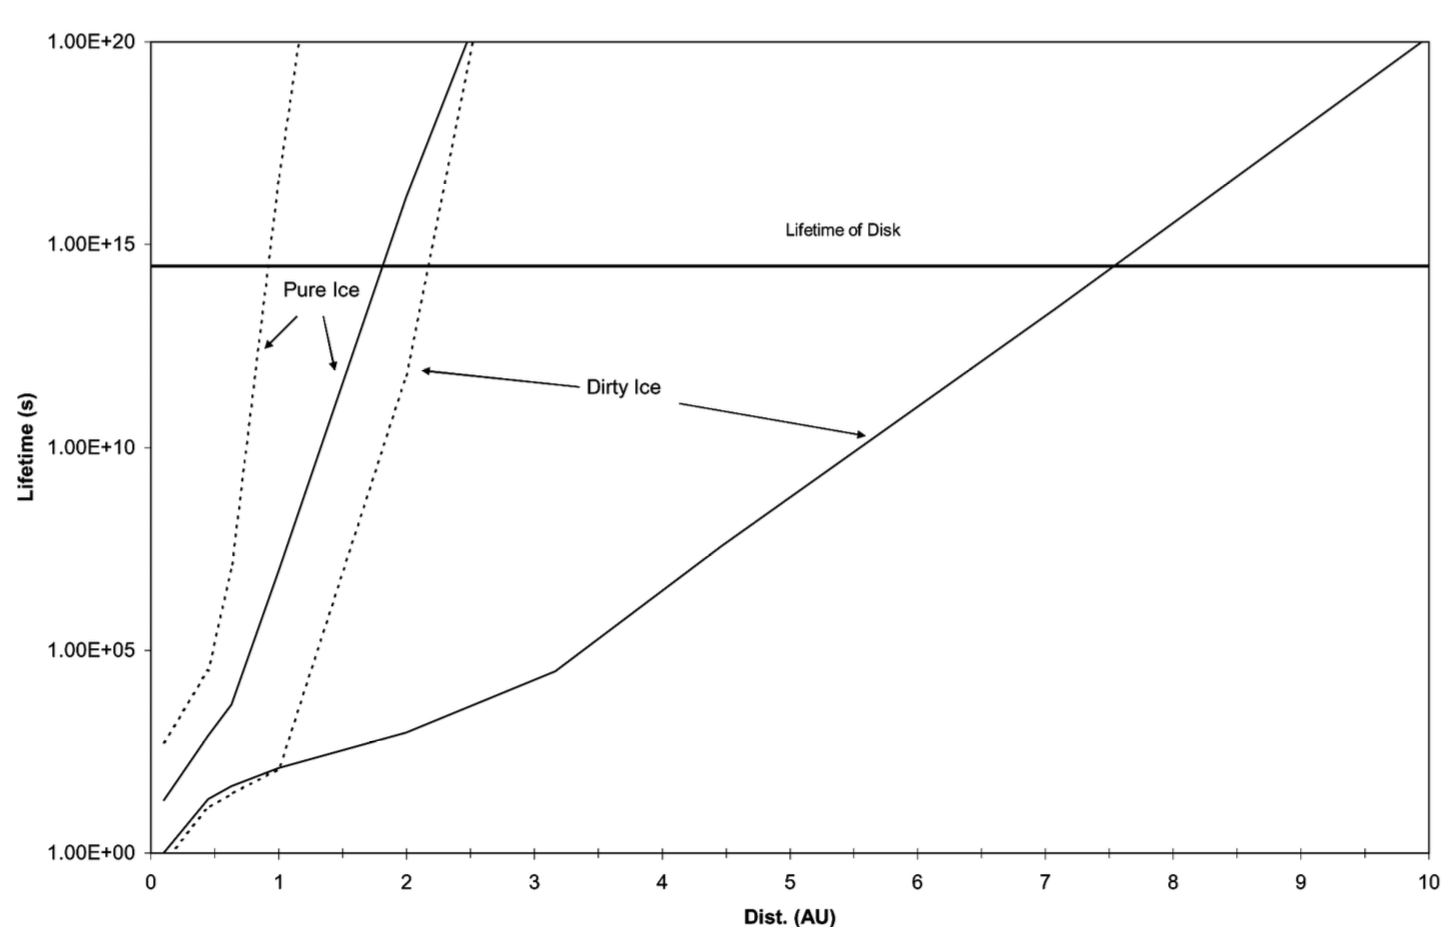
\includegraphics[width=0.7\textwidth]{figures/lifetime_water_ice}
	\caption{Comparison of lifetimes for pure and dirty ice grains. The dashed curves are for 0.1 $\mu$m grains and the solid curves are for 10 $\mu$m grains. The solid horizontal line shows a conservative upper limit to the age of the gas disk.  \cite{snow_line_age}}
	\label{fig::lifetimes_ice_grains}
\end{figure}


\subsection{D/H ratio in comets and asteroids}

The D/H ratio in comets and asteroids is linked to their formation region and therefore differs for various asteroids as well as comets from the Oort cloud and the Kuiper Belt and can be related to the D/H ratio in the solar nebula and the different planets. 
An overview of measured and estimated data is given in Figure \ref{fig::D_H_ratio_solar_system}

%\begin{figure}
%	\centering
%	\includegraphics[width=0.9\textwidth]{figures/D_H_ratio_outer_solar_system}
%	\caption{D/H ratios of various objects in the solar system.  \cite{constraints_comets_dhratio}}
%	\label{fig::D_H_ratio_outer_solar_system}
%\end{figure}

\begin{figure}
	\centering
	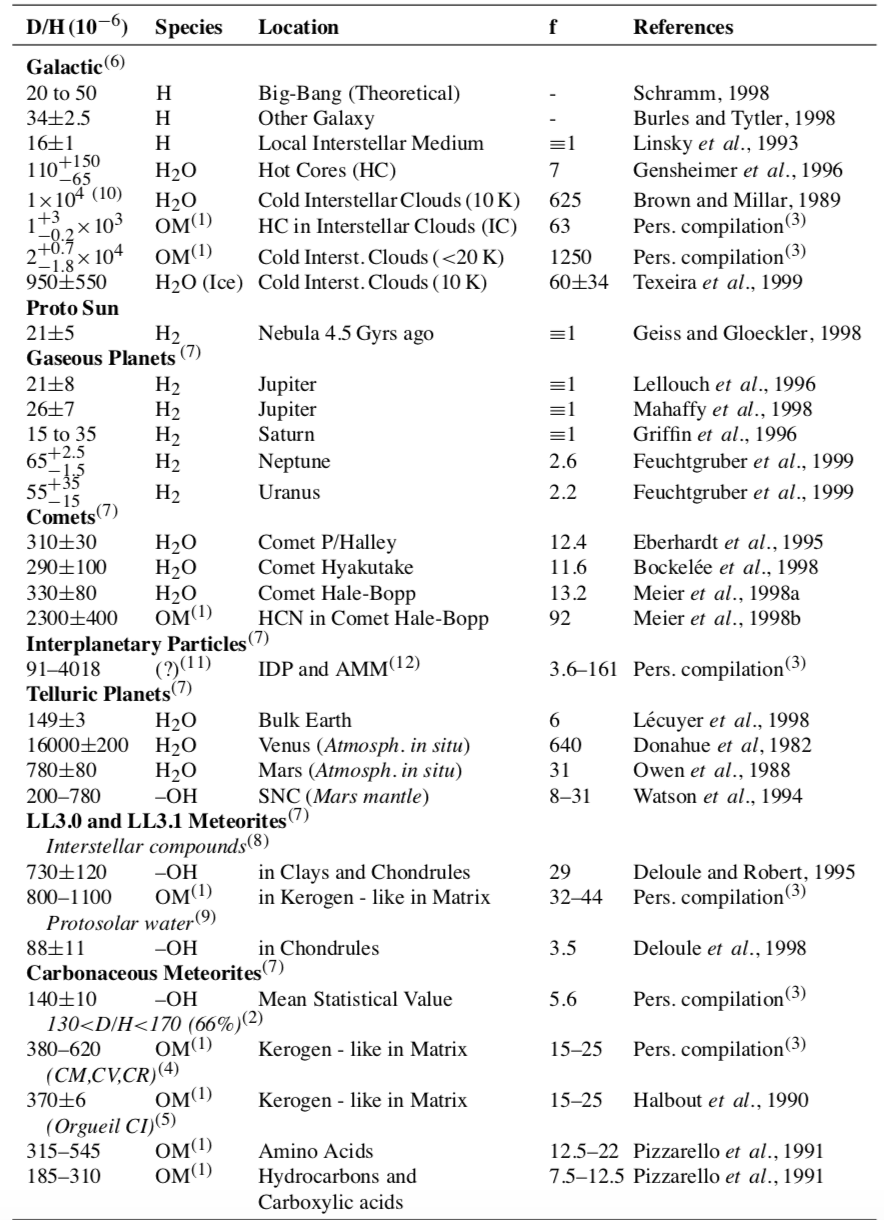
\includegraphics[width=0.9\textwidth]{figures/D_H_ratio_solar_system}
	\caption{D/H ratios of various objects in the solar system.  \cite{SolSystemDH_Robert}}
	\label{fig::D_H_ratio_solar_system}
\end{figure}

However, more recent observations of comet 103P/Hartley 2 have shown that it's H/D ratio is $(161 \pm 24) \times 10^{-6}$ and therefore significantly lower than estimated from previous measurements of other comets. This could be the case because the origin of 103P/Hartley 2 is not known for a certainty but it is believed that it could have originated in the Kuiper Belt, contrarily to a lot of other comets such as 1P/Halley who are widely believed to have originated in the Oort cloud. \cite{water_Hartley2_nature}

For comets it has been suggested that the deuterium enrichment factor depends on the creation epoch of the comet which is different for Kuiper Belt comets and comets from the Oort cloud, due to different temperature scales and depends on the evolution of the solar nebula over time. 

Using the enrichment factor $f$ for water
\begin{equation}
	f = \frac{1/2}{1/2} \frac{HDO/H_2O}{HD/H_2}
\end{equation}
which quantifies the D/H ratio for a certain deuteriated species, in this case water. As mentioned above, the deuterium enrichment factor $f$ depends on the temperature distribution of the isotopic exchange as well as the pressure distribution which is also temperature-dependent. The differential equation is given in Equation \ref{equ::diff_equ_f} \cite{transport_solar_nebula}:

\begin{equation}
	\partial_t f = \underbrace{k(T) P(A(T) - f)}_{\textrm{diffusion term}} + \underbrace{\frac{1}{\Sigma R} \partial_R (\kappa R \Sigma\partial_R f)}_{\textrm{exchange term}}
	\label{equ::diff_equ_f}
\end{equation}
$A(T)$ is the fractation at equilibrium, $P$ is the total pressure $R$ is the heliocentric distance, $k(T)$ is the isotopic exchange, $\Sigma$ is the gas surface density and $\kappa$ describes the turbulent diffusivity which depends on the nature of the turbulence. Equation \ref{equ::diff_equ_f} can be split up in an exchange and a diffusion term, the former describes the dependency of the heliocentric distance while the latter describes the dependency on the temperature distribution.

This connection is displayed and compared with measurement data from various comets in Figure \ref{fig::D/H_distance_age}.

\begin{figure}
	\centering
	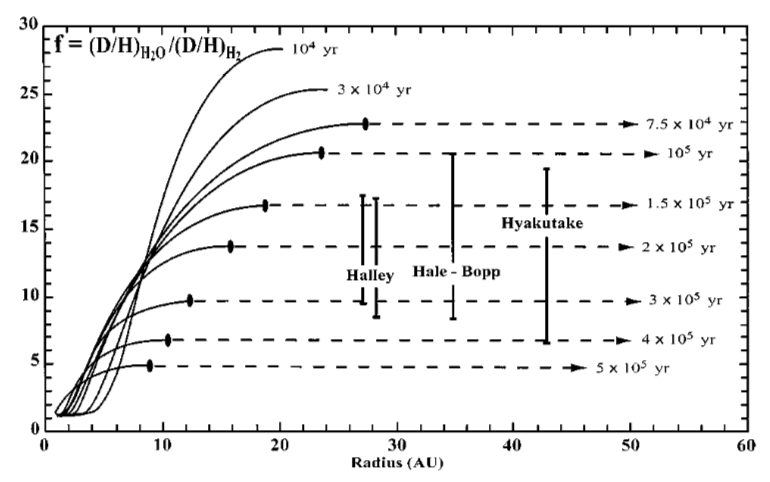
\includegraphics[width=0.5\textwidth]{figures/D_H_distance_time}
	\caption{Calculated deuterium enrichment factor f in H2O as a function of the heliocentric distance R, at various epochs in years of the evolution of the nebula. Dots indicate the heliocentric distance where H2O condenses. Dashed lines correspond to the value of f in ices. D/H enrichments obtained in comets Halley, Hyakutake, and Hale–Bopp are shown for comparison. The location of comets is arbitrary.  \cite{constraints_comets_dhratio}}
	\label{fig::D/H_distance_age}
\end{figure}


Meteorites with high D/H ratio are only those of the following two types: LL3 and carbonaceous chondrites. In both types, the insoluble organic matter shows elevated values of deuterium enrichment as well as clay minerals. The values obtained from the measurements of clay minerals can then be used to determine the D/H ratio of water because of the negligible isotopic fractionation between clay minerals and liquid water. \cite{SolSystemDH_Robert}


%\newpage
\subsection{Measurement data from 67P/Churyumov-Gerasimenko}
67P/Churyumov-Gerasimenko is a Jupiter-family comet that probably originated in the Kuiper Belt. During the Rosetta Mission detailed measurements of the D/H ratio were conducted, resulting in a D/H ratio of $(530 \pm 70)\times10^{-6}$, 3 times higher than the values found on Earth. Although 67P/Churyumov-Gerasimenko is expected to come from the same region of the Solar System as 103P/Hartley 2 (discussed in the previous section), they show significantly different values that suggest that the variety of Jupiter-family comets is greater than expected.  

\begin{figure}
	\centering
	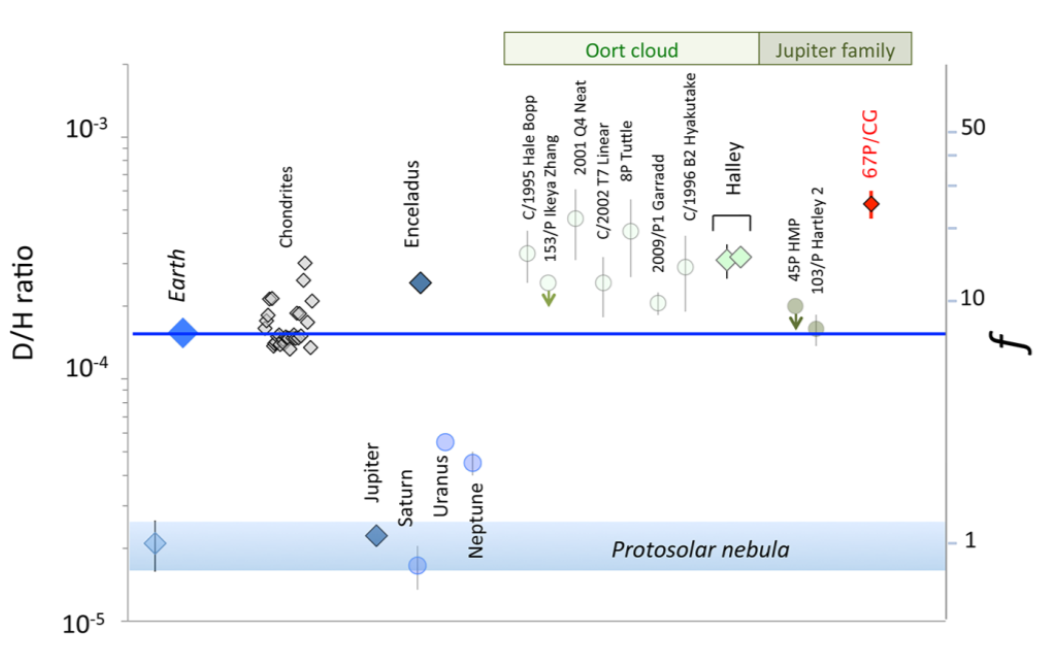
\includegraphics[width=0.6\textwidth]{figures/D_H_ratio_multiple_objects}
	\caption{D/H ratios in different objects of the solar system. Diamonds represent data obtained by in-situ mass spectrometry measurements, and circles refer to data obtained by astronomical methods. \cite{D/H_67P_science}}
	\label{fig::D/H_different_objects}
\end{figure}


%How/ where comets/ asteroids/ chondrites/ meteors are created and what this means for the d/h ratio (and perhaps other ratios) of those objects.\\
%State how the solar system formed + asteroids and comets (no terestial planets)\\
%Anja


%----------------------------------------------------------------------------------------
%	CHAPTER: FORMATION TERRESTRIAL PLANETS.
%----------------------------------------------------------------------------------------
\newpage
%----------------------------------------------------------------------------------------
%	CHAPTER: WATER CONTENT AFTER CREATION TERRESTRIAL PLANETS.
%----------------------------------------------------------------------------------------
\section{Water content of terrestrial planets after their creation}
There is currently no perfect explanation of how the terrestrial planets gained water. The most common hypothesis is that water arrived later on those planets because the temperatures were too high. Therefore the planets accreted dry. This hypothesis is researched in this chapter together with the less famous hypothesis that the planets were accreted wet. For the latter one, also the possibility of holding on to this water is researched.


%----------------------------------------------------------------------------------------
%	PARAGRAPH: FORMATION TERRESTRIAL PLANETS.
%----------------------------------------------------------------------------------------
\subsection{Formation of terrestrial planets in the early solar system}
The terrestrial planets formed from the protoplanetary disk, a large, cold and slowly rotating cloud of gas and dust. The gas and dust sometimes collided due to gravitational forces. If the collisions where gentle enough the gas and dust would grow into a bigger object and eventually into a protoplanet. The gas consisted mostly of hydrogen, helium and oxygen, some of the hydrogen and oxygen combined to make water vapor \cite[p.~523]{TPoriginWater}.\\

The amount of water vapor within 3 AU in the protoplanetary disk has been estimated at three earth masses \cite{TPLecluse} in 1994 and two earth masses \cite{TPPalme} \cite{TPLodders} in 2003. The mass of Earth is $5,9722 \pm 0.0006 \cdot 10^{27}$ g and the earth mass of all Earths oceans is $\pm 1,4 \cdot 10^{24}$ g. The amount of water inside the Earth is not exactly known, most estimations are around 10 Earth oceans with a extreme maximum of 50 Earth oceans \cite[p.~523]{TPoriginWater}. The water storage of Earth in minirals is about 5 - 6 Earth oceans \cite{TPOhtani}.\\

If all four terrestrial planets accreted with 50 Earth oceans of water, then that would still only be 4,7\% of the available water. There was probably enough water vapor in the early solar system to account for Earths oceans and the water on the other terrestrial bodies. The main problem is if the terrestrial bodies could hold on to this water during the formation of the protoplanets due to heat.


%----------------------------------------------------------------------------------------
%	PARAGRAPH: COULD THE TERRESTRIAL PLANETS HOLD ON TO THEIR WATER.
%----------------------------------------------------------------------------------------
\subsection{Water storage in terrestrial planets during formation}
There are two main possibilities of water being stored, hydrated minerals and absorption onto grains. The water can be depleted by high temperatures and collisions. In this paragraph the storage is studied. \\

There are hydrated minerals observed in the mid-asteroid belt. Some were apparently heated to several hundred degrees Celsius. This is a confirmation that water was present at the early solar system and can be stored. The hotter an asteroid would have been, the less of these minerals are found. The chances of the terrestrial bodies holding on to water in hydrated minerals are pretty slim because the temperature of those planets were much higher than those of the asteroids \cite{TPRivkin}.\\

There is also the possibility of water being absorbed by grains. Grains are small objects with a rough surface. The two forms of absorption that could have happened are physisorption and chemisorption \cite[p.~523]{TPoriginWater}. Physisorption is caused by the 'van der Waals force' which is $10 - 100$ meV $\approx 1,6 - 16 \cdot 10^{-21}$ J. Chemisorption involves a chemical reaction between the surface of the grain and in this case water. This force is stronger with $\approx 0,5$ eV $\approx 8 \cdot 10^{-20}$ J.\\

The effects of physisorption has been simulated by creating an Earth out of grains with a 100 times greater surface area than a spherical grain with the same volume. The finding were that with a temperature of 1000 K a quarter of Earths ocean could be absorbed. If the temperature would be 700 K than one Earth ocean would be absorbed and with 500 K three Earth oceans \cite{TPStimpf1} \cite{TPStimpf2}.\\

\newpage
If chemisorption is taken into account the force that keeps the water onto the grains will increase if there are multiple water molecules. How much it exactly contributes is unknown because tests are only performed at temperatures below 30 K. But it can be said that the force that keeps the water onto the grains will increase even at higher temperatures due to chemisorption \cite{TPchemistry}. \\

As the grains collide with each other, some or all of the water will be lost depending on the impact. In the physisorption simulation they accounted for this, if two grains collided with a force greater than two times the total bond energy. In that case all water would be gone. If chemisorption was also taken into consideration the total amount of water that could be stored in the proto-Earth would increase \cite{TPStimpf1} \cite{TPStimpf2}.


%----------------------------------------------------------------------------------------
%	PARAGRAPH: WOULD THE STORED WATER EVAPORRATE AFTER FORMATION.
%----------------------------------------------------------------------------------------
\subsection{Water loss in terrestrial protoplanets}
The early terrestrial planets probably melted one or multiple times while being accreted, probably from multiple major impacts, of which one created the moon. This means that there where magma oceans at some point in their lifetimes, before reaching their final solid state.  \cite{TPformationPlanetesimals}. \\

These magma oceans could have played a key role in delivering volatile into the growing atmosphere through degassing. For this to happen the magma ocean should have been over saturated by these elements and there was no boundary layer for these elements \cite[p.~128-129]{TPmagma}. \\

As the interior gained more heat the volatile elements broke down and formed bubbles that were being transported to the exterior. The melted material would become drier because most volatile elements would migrate to the atmosphere. Most of the big impacts would take away some of the Earths atmosphere but it could also bring other materials to Earth. The impacts would create more heat in the interior and the process of volatile elements out gassing continued until the interior was completely dry \cite[p.~130-131]{TPmagma}.\\

Due to the heat there could not be any oceans on Earth, but the Earth was massive enough to keep most water vapor in the atmosphere. After the Earth cooled down this vapor could condense and become Earths first oceans. Through plate tectonics and volcanic activity more water could be transported from inside the Earth to the oceans \cite[p.~130-131]{TPmagma}.


%----------------------------------------------------------------------------------------
%	PARAGRAPH: D/H RATIOS OF (TERRESTRIAL) PLANETS
%----------------------------------------------------------------------------------------
\newpage
\subsection{The current D/H ratio of terrestrial planets}
The distribution of the D/H ratio through the solar system can be seen in figure \ref{fig:dh-ratio-terrestrial-planets}. It's clear that how further away from the sun, the higher the D/H ratio. Mars has a D/H ratio which is 7 times larger and Venus has a D/H ratio which is 150 times larger. The latter one is a discrepancy because Venus is closer to the sun than Earth. It's possible that Venus got more water from comets from far way in the solar system. This confirms that the origin of water is from comets. Another explanation is that the ultraviolet radiation from the sun breaks water molecules into H and OH, the lighter gass will escape into space. It is possible that Venus lost an ocean’s worth of water but Earth did not because Earth was too far from the Sun for the instability to develop \cite{TPthreeEras}.

\begin{figure}[H]
	\center
	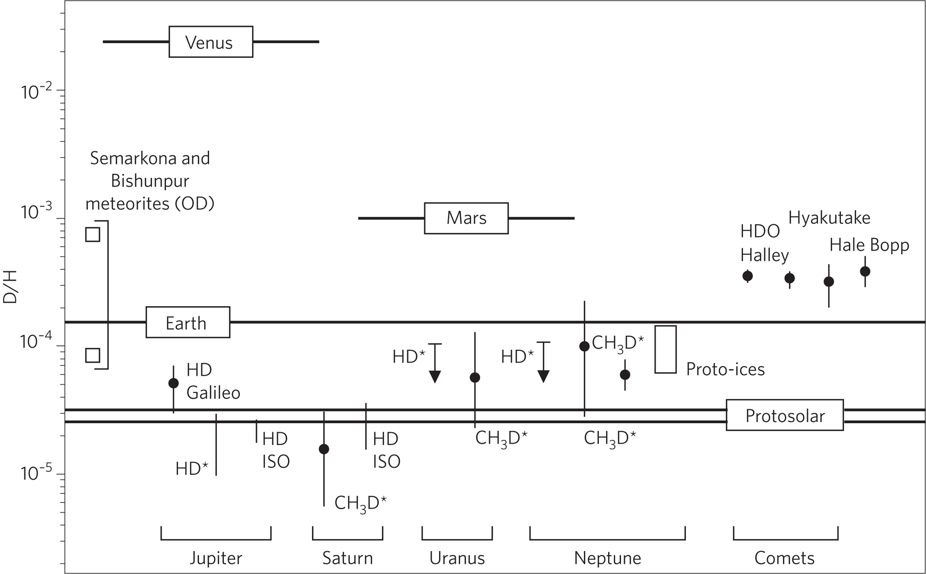
\includegraphics[width=0.75\textwidth]{figures/dh-ratio-terrestrial-planets.jpg}
	\caption{\label{fig:dh-ratio-terrestrial-planets}D/H ratio in the solar system \cite{TPthreeEras}.}
\end{figure}




%----------------------------------------------------------------------------------------
%	CHAPTER: BOMBARDMENT EARTH.
%----------------------------------------------------------------------------------------
\newpage
%----------------------------------------------------------------------------------------
%	BOMBARDMENT OF EARTH.
%----------------------------------------------------------------------------------------

\section{\label{chap:bombardment}The bombardment of Earth}
There are differing trains of thought on the timing, how and where the Earth received its water. The two possibilities where water could come from are either through internal reserves acquired during the accretion process or from extraplanetary sources after Earth’s development. These extraplanetary sources of water would have come from asteroids, comets and protoplanet collisions. The hypothesis that concerns these objects delivering water to a developed and dry Earth is referred to as the late heavy bombardment. The hypothesis that Earth’s water comes from extraplanetary origins is not flawless and has controversy. There is another hypothesis where the water was accumulated during the Earth’s accretion development. This hypothesis is referred to as the “Accretion Model”. These are the two base theories about the origin of Earth’s water. These hypotheses have evolved over time to account for previously unknown scientific data.

\subsection{Late Heavy Bombardment}
The Late Heavy Bombardment has been addressed by different names such as “Late Veneer”, “Late Bombardment Hypothesis”, “Late Accretion”, and “Late Heavy Bombardment”: for consistency within this report, this hypothesis will be referred as “Late Heavy Bombardment” or LHB. The late heavy bombardment has variations that cover the various objects that could deliver water to the Earth as well as the influences of different planetary orbits. The various objects included are comets, asteroids and planetesimals. The time frame of this bombardment happened between 4.4 and 3.5 Ga \cite{LHB_Timeframe}. This hypothesis was first noted by Hopp\cite{BOMB1} but not named as such in an article from Kimura et al. concerning the discrepancy in gold distribution \cite{BOMB2}. However, another article from Maruyama \cite{BOMB3} report that another article written by E. Anders \cite{BOMB4} first came up with the theory. The start and progression of this theory concerns the siderophile elements and their distribution within the Earth. The elements include tungsten, ruthenium, gold, osmium, iridium, and more elements \cite{BOMB5} \cite{BOMB6} \cite{BOMB7}. These reports on the different elements shows the gathering of data for this hypothesis. The late heavy bombardment has competing views on the origin of Earth’s water. The most popular to least popular opinions are asteroids, comets and then planetesimals. There are reports and articles \cite{BOMB8} \cite{BOMB9} \cite{BOMB10} that highlight the differences between the sources as well as likelihood and the effects coming from the different sources. The most commonly discussed of these sources are the carbonaceous chondrite asteroids. The asteroids are the viewed as the most likely source of the Earth’s Water in the late heavy bombardment.

\subsubsection{Comets}
Comets have showered Earth in dust and ice in their wake and the occasionally impact on Earth. 
There are two classes of comets: short period and long period comets. 
The distinction is whether their orbital period is less or greater than 200 years. 
The long period comets are from the Kuiper Belt and the Oort Cloud while the short period comets are from the Jupiter and Saturn Belt.
With the discovery of comets comprising significantly of water, comets were the first extraplanetary objects to be considered as the source of Earth's water. The impact of comets could deliver significant amount of water and would effect Earth's climate and atmosphere.

\newpage
\paragraph{Probability and Numbers}
Comets are abundant in the solar system. Estimates of the number of comets in the solar system are in the magnitudes of \(10^{11}\sim 10^{12}\) objects \cite{Comet_Num}.The current amount of comets is approximately one-fifth of the original amount of comets \cite{Comet_AvgSz}. The amount of comet material could amount to almost \(2\%\) \cite{Comet_AvgSz} the solar system mass. However scientists have only been able to observe under \(6000\) \cite{observed_objects} comets and explored and studied only a handful of comets.


The mass of comet 67P is \(9.98 \times 10^{12}\)kg \cite{67P_Mass} with water ice accounting for \(75\%\) \cite{67P_Water} of the comet which corresponds to \(7.48 \times 10^{12} kg\).
Comet Halley is \(2.2 \times 10^{14}kg\) \cite{Cevolani1987} and contains \(40\% \) water ice \cite{Comet_Yeomans} by weight. The comet Halley should have \(8.8 \times 10^{13} kg\) of water ice.
Assuming average spherical size and density of short period comets are 4.4 kilometers \cite{Comet_AvgSz} and \(0.6 \: \sfrac{g}{cc}\) \cite{Britt2006SmallBD} respectively meaning an average mass of \(2.14 \times 10^{14}kg\). Assuming similar hydration levels as come Halley with 40\% water ice by weight, an average comet would hold about \(8.56 \times 10^{13}kg\) kg of ice.

Under ideal conditions of perfect transfer of all material from the comet to the Earth and no loss of previously accumulated water, it would take almost 180 million comets to provide Earth its \(1.54\times 10^{22} kg\) of water. A total of \(3.85\times 10^{22} kg\) of comets would be needed for this set of ideal conditions.

Assuming non-ideal conditions, such as, an non perfect transfer on water and non-negligible of previous water  due to the impact. The amount of water accumulated will not reach the desired value of \(1.54\times 10^{22} kg\), this is due to the loss of previous water being equal to the amount of water transferred to Earth as the assumed average comet is not large enough to transfer more water than the Earth would have lost to space.

\paragraph{Controversy and Disagreements}
The hypothesis of comets being the source of water on Earth is not without contention. The main points that cause scientist to disagree with this assertion are the deuterium to hydrogen ratios and the time frame of the bombardment from Jupiter's comets.
The comet deuterium hydrogen ratios are much higher than Earth's, especially with comet 67P being 3 times the value of Earth's. 
The second point that causes disagreements which includes Jupiter's development into the equation of scattering comets and asteroids towards Earth. Comets were most likely scattered within a million years after Jupiter was fully developed, and at that point of time in the solar system, the Earth was a much smaller target \cite{morbidelli2000source}. 
These arguments against tend to discount comets being a main source of water for Earth.

\paragraph{Conclusion}
Comets are bountiful objects of ice and dust that people throughout the ages can admire or fear. They did deliver ice and other volatile elements to Earth through collisions.
There is enough cometary mass in the solar system to provide Earth the required amount of water. 
However due to the issue with the size of the planet at the time of bombardment and the high deuterium to hydrogen ratio, scientists have stated that this is improbable source.
The high deuterium to hydrogen ratio found in comets, some scientists speculate that at most 10\% of the Earth's water comes from comets \cite{morbidelli2000source}.
Comets have contributed to Earth's water but in a minor role rather than the primary contributor.

\subsubsection{Asteroids}
Asteroids are becoming the popular origin of water on Earth.
Asteroids are different from comets, both in origin location and composition.
The asteroid belt can be separated by the the Kirkward gaps at 2.5 and 2.82 AU\cite{AsteroidBelt}, into the inner, middle and the outer asteroid belt.
These inner belt has differing properties compared to the middle and outer belts with the most notable in this report being hydration values.

\paragraph{Calculations and Associated Probability}
The inner asteroid belt is much dryer with an hydration of \(<0.1\%\) by weight while the  asteroid belt beyond 2.5 AU contains more water with up to \(10\%\) by weight \cite{morbidelli2000source}. The sizes of asteroids range from meters to hundreds of kilometers large with the asteroid belt being composed of asteroids smaller and larger than 1 kilometer in size \cite{asteroid_AvgSz}. The average density of an asteroid depends on its classification, the densities varies from \(1.38 \: \sfrac{g}{cc}\) for carbonaceous, \(2.71 \: \sfrac{g}{cc}\) for silicate, and \(5.32 \: \sfrac{g}{cc}\) for metallic asteroids\cite{AsteroidBeltMass}. 

With an estimate of 1 kilometer sized asteroid with an averaged density of \(3.1 \: \sfrac{g}{cc}\)and assuming the hydration to be \(0.1\%\) for inner belt asteroids and \(10\%\) for middle and outer belt asteroids.
In Ideal transfer of perfect mass capture and negligible previously retained water escaping due to the collision, the amount of inner belt asteroids to collide with Earth would be just under 1 trillion asteroids to give Earth its \(1.54\times 10^{22} kg\) of water. This amount of asteroids is problematic as it is more than twice the mass of planet Earth at \(1.5\times 10^{25} kg\).
It would take 10 billion middle and outer belt asteroids with a combined mass of \(1.5\times 10^{23} kg\) or \(2.5\%\) of Earth's mass.
The current asteroid belt has \(3.58 \times 10^{21}kg\) \cite{AsteroidBeltMass}.
It is hypothesized that the current asteroid belt is a remnant compared to the primordial asteroid belt at 1\% its former size \cite{PrimAstBelt}. If using the former size, there is sufficient material if all the asteroids were well hydrated.

\paragraph{Controversy and Disagreements}
There is not a consensus on if asteroids is the origin of water on Earth. One of the issues that cause contention is Jupiter's influence on the asteroid belt. Jupiter's influence on the scattering of the primordial asteroid belt would have been too early. Morbidelli concluded that the large majority of asteroids would collide with the Earth before the Earth was 60\% formed \cite{morbidelli2000source}. 
There is also a contention on the primordial asteroid belt size, with a new hypothesis stating that it was empty and was filled instead of losing nearly all of its objects \cite{Emptybelt}. This would prevent asteroids being the source of water as there would have not been any to deliver water to the Earth.
The primordial belt if two magnitudes larger than today's value would have a similar variation of hydration and would not deliver the needed amount of water on Earth.

\paragraph{Conclusion}
Asteroids are considered the leading explanation for water on Earth. 
The deuterium to hydrogen ratio of asteroids are much closer to Earth's values than comet's. 
However this scenario still leaves much to desire as the primordial asteroid belt might not have significant enough amount of water to hydrate the Earth.

\subsubsection{ABEL Model}
The new hypothesis in Late Heavy Bombardment is ``Advent of Bio-ELements" (ABEL) model\cite{ABEL_1}. 
ABEL attempts to reconcile evidence of water within the Earth with LHB. ABEL model comprises of a two step process: Earth was formed dry with no atmosphere or oceans then gained an atmosphere and oceans. 

\newpage
\paragraph{Differences between ABEL and other LHB}
ABEL model considers multiple geological characteristics compared to the previously described Late Heavy Bombardment scenarios. 
The late bombardment that occurred in the middle of Hadean era is renamed to the ABEL bombardment.
ABEL model considers the origin of plate tectonics and the presence of water within the Earth which is not considered within the previous models. 
The areas that ABEL differs from that of the cometary, asteroidal or planetesimal scenarios are having no atmosphere, a rigid lithosphere, and a completely reductive planet \cite{ABEL_1}.

ABEL model states that the Earth originally formed without an atmosphere. The atmosphere was developed during the ABEL bombardment with the presence of volatiles and water. The bombardment provided the oceanic and atmospheric elements to the dry Earth \cite{ABEL_2}.

A large concentration of ABEL is the plate tectonics. The model proposes that there was a large solid lithosphere \cite{ABEL_2}. The ABEL bombardment with massive asteroids broke and subducted the primordial continents into the mantle as well as  introducing volatiles which is needed for plate tectonics \cite{ABEL_3}. 

\subsubsection{Effects of Late Heavy Bombardment}
The impacts from extraplanetary object have significant effects on the planet Earth.
The consistent impacts consistent with LHB would produce large lava oceans, up to 10\% of Earth's surface  and would have increased the temperature significantly and possibly evaporate all the oceans \cite{LavaOcean}.
The impacts would have caused massive amounts of rock dust and water vapor to enter the high atmosphere. The sub-micrometer dust cloud can severely block incoming light from the sun and cool the planet, and the water vapor may be photolyzed and be lost to space \cite{ImpactDust}. 
These are very harsh environments for life to form from.


\subsection{Conclusion}
The main two hypotheses are the Late Heavy Bombardment and the early accretion model. The Late Heavy Bombardment says that Earth was formed dry and received water and volatiles from extraplanetary sources. This model dismisses all claims from the early accretion model concerning the possibility of the Earth forming wet. The early accretion model does not preclude the Late Heavy Bombardment, however does severely limit the amount of water accumulated from extraplanetary sources. There is agreement on “our knowledge of detail of terrestrial planet formation and hydration is currently insufficient” \cite{BOMB14}.





%The current amount of water in asteroids is quite low (way lower than comets). Were there enough asteroids to deliver the water to Earth?\\
%Wouldn't a comet/asteroid heat up the atmosphere so much that most of the vapor won't get stuck in Earths atmosphere?\\
%Where did those asteroids/comets come from?\\
%Adam


%----------------------------------------------------------------------------------------
%	CONCLUSION.
%----------------------------------------------------------------------------------------
\newpage				% Start at new page.
%----------------------------------------------------------------------------------------
%	CONCLUSION & RECOMMENDATIONS.
%----------------------------------------------------------------------------------------

\section{\label{chap:conclusion}Conclusion \& Recommendations}

The era of the origin of Earth has plenty of mysteries and questions remaining to be answered. One of the most important of these questions is about the origin of water on this planet. The answer to this question would reveal how life started to exist and on how other terrestrial planets in other solar systems might develop. This question of the origin of water has been asked and tried to have a satisfactory answer for several decades, no answer has been completely satisfactory. The The main two hypotheses are the Late Heavy Bombardment and the early accretion model. 
The Late Heavy Bombardment says that Earth was formed dry and received water and volatiles from extraplanetary sources. This model dismisses all claims from the early accretion model concerning the possibility of the Earth forming wet. 
The early accretion model does not preclude the Late Heavy Bombardment, however does severely limit the amount of water accumulated from extraplanetary sources. 
The issues with Late Heavy Bombardment is that the isotopes of comets do not match Earth's deuterium to hydrogen ratio; the asteroids have issues with the quantity of hydrated materials. 
The Early Accretion model has issues with retention of water in during the development process.
There is agreement on “our knowledge of detail of terrestrial planet formation and hydration is currently insufficient” \cite{BOMB14}. 

There has been research and modeling that shows only physical absorption or chemical absorption. There should be new research focus on the combination of those two absorption methods to model how much water would be absorbed into grains and minerals. 
The model should determine whether the grains and hydrated minerals would retain water at elevated temperatures that are seen during the development of terrestrial planets.
There should be further research into seeing if the minerals and dust can retain their water at the pressure associated with the impact nature of accretion.
With more research there can be a possible evidence or discrepancy that could make one scenario more or less likely to have occurred.



%----------------------------------------------------------------------------------------
%	RECOMMENDATIONS
%----------------------------------------------------------------------------------------
\newpage				% Start at new page.
%----------------------------------------------------------------------------------------
%	RECOMMENDATIONS.
%----------------------------------------------------------------------------------------

\section{Recommendations}
What can we do/measure to get more information about the origin of water.


%----------------------------------------------------------------------------------------
%	REFERENCES.
%----------------------------------------------------------------------------------------
\newpage				% Start at new page.
\addcontentsline{toc}{section}{References}
\bibliographystyle{ieeetr}
\bibliography{references}


\end{document}